\section{Introduction}
Time variation in higher moment parameters has received a growing interest in the past decade, as research has shifted focus on capturing extreme market
movements which have appeared to occur with a degree and frequency not typically expected by traditional models. The popular GARCH family of models,
while able to produce thick-tailed and skewed unconditional distributions under certain assumptions and parameterizations, typically assume
that the shape and skewness parameters are time invariant. This also leads to the assumption that the conditional distribution of the standardized innovations
is independent of the conditioning information, for which there is no good reason to believe so a-priori. Different models have been developed in the literature to
capture dependencies in higher moments, starting with \citet{Hansen1994} who considered the problem of modelling the full parameters of a generalized
skew-student distribution by imposing a quadratic law of motion on the conditioning information. With few exceptions, the research on time varying
higher moments has mostly explored different parameterizations, in terms of dynamics and distributions, with little attention to the performance of these
models out-of-sample or in their ability to outperform GARCH models with respect to such measures as Value at Risk (\emph{VaR}) which are important in
risk management. In addition, estimation of such models has been plagued by problems introduced by the bounding transformation of the higher moment distribution
parameters, and multivariate extensions, when they have been considered, have been completely infeasible for large scale applications.\\
The \verb@racd@ package aims to provide for a feasible and (almost) painless modelling environment for working with these models, offering a good choice of
motion dynamics for the moments and a wide choice of conditional skewed and shaped distributions. Methods for estimation, filtering, forecasting and simulation are
provided with the same uniform extractor methods as in the \verb@rugarch@ package. Because the \verb@racd@ extends the \verb@rugarch@ package, it is expected
that the user is familiar with that package, and any gaps in the current documentation can likely be filled by reference to that.\\
The \verb@racd@ package is currently hosted on the \verb@rugarch@ Google code development site (\url{http://code.google.com/p/rugarch}) and there are no plans
for releasing to CRAN. This vignette hopefully provides enough details about working with the higher moment models, but because of the estimation challenges,
and the advanced nature of the models, particular care should be used. If you have questions, use the R-SIG-FINANCE mailing list to ask them (there is no guarantee
of an answer) and DO NOT send me private emails asking for support (I will most likely ignore them, with few exceptions). Finally, a comprehensive example
demonstrating the use of the package is available on my website (\url{http://www.unstarched.net}).\\
The package is provided AS IS, without any implied warranty as to its accuracy or suitability. A lot of time and effort has gone into the development of this
package, and it is offered under the GPL-3 license in the spirit of open knowledge sharing and dissemination. If you do use the model in published work
DO remember to cite the package and author (type \verb@citation@("racd") for the appropriate BibTeX entry) , and if you have used it and found it
useful, drop me a short note and let me know.
\section{Literature Review}
Estimation of ACD models has traditionally been a very hard exercise, because of the highly nonlinear bounding transformation for the higher moment distribution
parameters, their possibly joint interaction in determining the moments of the distribution, and the single source of noise driving these and the volatility
process. In \citet{Harvey1999}, \citet{Brooks2005}, \citet{Premaratne2000}, \citet{Rockinger2002} and \citet{Jondeau2003} for example,
different laws of motion and distributions for modelling the full time varying conditional density parameters were considered, on instruments varying from real
estate to foreign exchange returns. The results were mixed, with \citet{Harvey1999} finding significant evidence of time varying skewness,
\citet{Jondeau2003} finding both time varying skewness and kurtosis significant, while \citet{Premaratne2000}, \citet{Brooks2005}
and \citet{Rockinger2002} found little evidence of either. With regards to the frequency of observation, \citet{Jondeau2003} found the
presence of time varying skewness and kurtosis in daily but not weekly data, partly consistent with the observation that excess kurtosis diminishes with
temporal aggregation, while others including \citet{Hansen1994}, \citet{Bond2003} and \citet{Harvey1999} did find evidence of time varying
skewness  and kurtosis in weekly and even monthly data. The algorithmic challenges of estimating time varying higher moments was emphasized in
\citet{Bond2003} who argued that model convergence problems likely arose because of the constraints required to limit the distribution parameters
within certain bounds and the fact that both skewness and kurtosis are driven by extreme events making their identification with a particular
law of motion and (standardized) residuals very hard. Reading through the numerous revisions of the the paper by \citet{Jondeau2003}, it becomes
clear how difficult the estimation of these models has been. Originally, these authors tried to constrain the dynamics directly at every point in time
using an SQP solver with as many constraints as there were time points. Realizing that this would not guarantee the distribution bounds in out of sample
forecasting, they experimented with different dynamics, bounding transformations and Bayesian estimation. Though their numerous publications on
time varying higher moments has attempted to highlight what they call the value of distributional timing, their multivariate
extensions remain difficult to estimate and suffer from significant dimensionality issues ( see for example \citet{Jondeau2012} ).\\
The distributions used in the ACD literature have mostly been limited to some variation of the Student distribution. For example, \citet{Hansen1994}
and \citet{Jondeau2003} have used the Generalized Student distribution, \citet{Harvey1999} the noncentral Student distribution, \citet{Lambert2001} a
skewed Student distribution, while \citet{Brooks2005} a standard Student distribution to model only kurtosis. Departures from the Student variations
have included a Pearson Type IV distribution in \citet{Brannas2003}, an Entropy distribution in \citet{Rockinger2002} and the non-parametric Gram-Charlier
expansion of the Normal as in \citet{Leon2005}, the properties of which were analyzed more fully in \citet{Jondeau2001}. More recently, \citet{Wilhelmsson2009}
used the NIG distribution with ACD dynamics in a risk management exercise using a long history of the daily returns of the S\&P500. In GARCH and ACD models,
the actual choice of distribution, beyond the key modelling requirements (such as possessing the scaling property), should be guided by such features
as the existence of a multivariate extension and the domain of variation of its higher moments. The latter feature is also related to the problem of
the existence of moments\footnote{For distributions with unbounded support, this is the Hamburger moment problem.}, where it can be shown that
for a density to exist, $Kurtosis > {Skewness^2} + 1$ (for strictly positive Kurtosis). An interesting way to visualize this is via an authorized
domain plot, available in the \verb@rugarch@ package via the \emph{skdomain} function and illustrated for a number of distributions in
Figure \ref{fig:skdomain}. It is clear from the figure that the skew Student distribution has the widest possible combination of skewness
and kurtosis for values of kurtosis less than $\sim 6$, whilst the NIG has the widest combination for values greater than $\sim 8$. It is interesting
to note that the Hyperbolic distribution is not defined for values of kurtosis greater than $\sim 9$. Finally, it should be noted that whilst Johnson's SU
appears to offer a competitive distribution to the NIG, and has a density representation which is simpler (and hence faster to evaluate the likelihood),
it does not unfortunately posses a standard multivariate extension.\\
\begin{figure}[!ht]
\centering
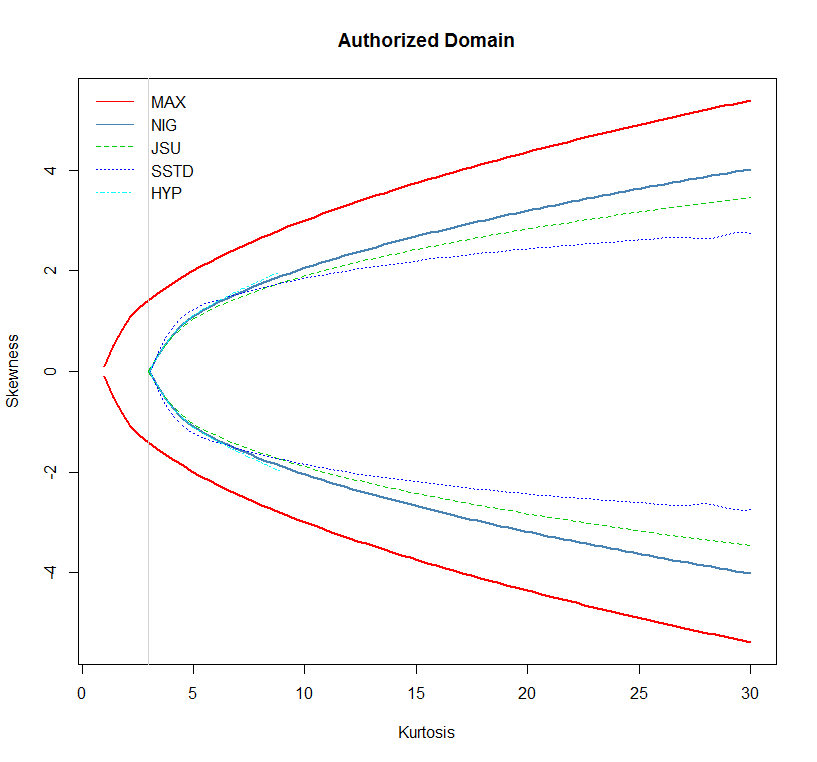
\includegraphics[width=10cm]{skdomain.png}
\caption[Authorized Domain of Skewness-Kurtosis]{Authorized Domain of Skewness-Kurtosis}\label{fig:skdomain}
\end{figure}
With few exceptions, out of sample performance evaluation of ACD models with respect to applied measures such as VaR has been limited. The vast majority of
papers reviewed simply investigated the in-sample dynamics of the models, inferring from the estimated parameters the presence or absence of time variation
in the higher moments without attempting to address the issue of how this translates, out-of-sample, to a value added input in an applied setting. Notable
exceptions have included \citet{Wilhelmsson2009} who used an ACD-NIG model against 4 other models including the model of \citet{Hansen1994}, and 3 GARCH models,
within a risk management application on the S\&P 500 index going back to 1962. The S\&P 500 index was also the choice for an intraday model using VaR and
Expected Shortfall with a time varying skewness model by \citet{Ergun2010a}. In both studies, the ACD models outperformed the non-time varying models on
some measures, though it was difficult to obtain very strong endorsements of this. More clear results have been found in multivariate extensions, with the
IFACD model of \citet{Ghalanos2013} providing for large scale feasible estimation with many desirable properties such as analytic representation of
higher co-moments and semi-analytic representation of the weighted portfolio density.\\
The \verb@racd@ package includes a diverse and varied set of conditional skew and shaped distributions for modelling time varying higher moments, including
the Generalized Hyperbolic and sub-families (including the NIG and GHST as separate implementations for reasons of speed), Johnson's SU (see \citet{Johnson1949})
and the skewed distributions arising from the inverse scale factor transformations described in \citet{Fernandez1998}, with a number of different motion dynamics
for the higher moment parameters, and discussed in the next section.
\section{Background}\label{sec:background}
The Autoregressive Conditional Density (\emph{ACD}) model\footnote{Also abbreviated as \emph{ARCD} in the literature, whilst \emph{ACD} has also been used for the Autoregressive Conditional
Duration model of \citet{Engle1998}.}, formally introduced by \citet{Hansen1994}, generalizes GARCH type dynamics to time varying conditional higher moments and as such subsumes them. In GARCH models, the density function is usually written in terms of the location and scale parameters, normalized to give zero mean and unit variance. The same arguments follow in ACD models, and I follow the exposition of \citet{Hansen1994} and consider the density function $f(y|\alpha)$, partitioned so that
\begin{equation}\label{eq:garchdensity1}
{\alpha _t} = \left( {{\mu _t},{\sigma _t},{\eta _t}} \right),
\end{equation}
where the conditional mean is given by
\begin{equation}\label{eq:garchdensity2}
{\mu _t} = \mu \left( {\theta ,{x_t}} \right) = E\left( {{y_t}|{x_t}} \right),
\end{equation}
and the conditional variance is,
\begin{equation}\label{eq:garchdensity3}
\sigma _t^2 = {\sigma ^2}\left( {\theta ,{x_t}} \right) = E\left( {\left( {{y_t} - {\mu _t}^2} \right)\left| {{x_t}} \right.} \right),
\end{equation}
with ${\eta_t} = \eta(\theta ,{x_t})$ denoting the remaining parameters of the distribution, such as a shape and skew parameter. The conditional mean and variance are used to scale the innovations,
\begin{equation}\label{eq:garchdensity4}
{z_t}\left( \theta  \right) = \frac{{{y_t} - \mu \left( {\theta ,{x_t}} \right)}}{{\sigma \left( {\theta ,{x_t}} \right)}},
\end{equation}
having conditional density which may be written as,
\begin{equation}\label{eq:garchdensity5}
g\left( {z|{\eta_t}} \right) = \frac{d}{{dz}}P\left( {{z_t} < z|{\eta_t}} \right),
\end{equation}
and related to $f(y|\alpha)$ by,
\begin{equation}\label{eq:garchdensity6}
f\left( {{y_t}|{\mu _t},\sigma _t^2,{\eta_t}} \right) = \frac{1}{{{\sigma _t}}}g\left( {{z_t}|{\eta_t}} \right).
\end{equation}
The difference between ACD and GARCH models is that in the latter case, $\eta_t$ is time invariant. In GARCH models the conditional density of the standardized residuals is constant while the residuals have a time varying conditional density arising as a result of the scaling from the GARCH volatility. In ACD models on the other hand, the conditional density of the standardized residuals is itself time varying as a result of the higher moment parameter dynamics, and the conditional density of the residuals has time variation arising from both the latter and the scaling from the volatility.\\
A first order constant-GARCH(1,1) model with ACD dynamics for the skew ($\rho_t$) and shape ($\zeta_t$) parameters can be represented as,
\begin{equation}\label{eq:acd1}
\begin{gathered}
  {x_t} = {\mu _t} + {\varepsilon _t} \hfill \\
  {\varepsilon _t} = {\sigma _t}{z_t} \hfill \\
  {z_t}\sim \Delta \left( {0,1,{\rho _t},{\zeta _t}} \right) \hfill \\
  \sigma _t^2 = \omega  + {\alpha _1}\varepsilon _{t - 1}^2 + {\beta _1}\sigma _{t - 1}^2 \hfill \\
  {\Phi}\left( {{\rho _t}} \right) =  {f}\left( {{{\bar \rho }_t}} \right) \hfill \\
  {\Phi}\left( {{\zeta _t}} \right) = {g}\left( {{{\bar \zeta }_t}} \right) \hfill \\
\end{gathered}
\end{equation}
where $\Delta$ is some appropriately scaled (0,1) distribution having a skew and shape parameter, $\Phi(.)$ represents some appropriate transformation function to the unconstrained motion dynamics of those parameters (denoted by a bar), constraining them within their distribution specific bounds, and $f$ and $g$ the motion dynamic functions for those parameters. Contrary to variance, which is directly modelled and constrained to be positive, the modelling of higher order moments is done indirectly via the some distributional parameters which usually have to be constrained within a specific range. The shape parameter(s) controls the tail thickness while the skew parameter(s) the asymmetry, and both may be needed in the calculation of the higher order central moments such as skewness and kurtosis. The ACD model can be modelled with any type of dynamics for the variance, and higher moment parameters, but because of the varying nature of the latter only certain types of dynamics will immediately lead to closed form solutions for persistence in the conditional variance equation, while for the higher moments only simulation methods are available to evaluate the unconditional moments, when these exist. For the simple model given above, the persistence and unconditional value of the variance are easily derived from the literature on ARMA type processes, and useful for imposing some stationarity conditions during estimation and for n-ahead forecasting,
\begin{equation}\label{eq:acd3}
\begin{gathered}
  E\left( {\sigma_t^2} \right) = \frac{\omega }
{{1 - \left( {{\alpha _1} + {\beta _1}} \right)}}, \hfill \\
  E\left( {{\eta_t}} \right) \equiv E\left( {\Phi \left( {{{\bar \eta}_t}} \right)} \right), \hfill \\
\end{gathered}
\end{equation}
which because of the nonlinear transformation, $E\left( {\Phi \left( {{{\bar \eta }_t}} \right)} \right) \ne \Phi \left( {E\left( {{{\bar \eta }_t}} \right)} \right)$.
As a result, the unconditional value of the higher moment parameters, and hence the higher central moments, must be estimated via simulation.
In the original model of \citet{Hansen1994}, first order quadratic type dynamics were used for the higher order parameters:
\begin{equation}\label{eq:acdquad1}
{{\bar \eta }_{t}} = {c_0} + {c_1}{z_{t - 1}} + {c_2}z_{t - 1}^2 + {d_1}{{\bar \eta }_{t - 1}},
\end{equation}
while \citet{Jondeau2003} used, among other tested parameterizations, first order piecewise linear dynamics:
\begin{equation}\label{eq:acdpwl1}
{{\bar \eta }_{t}} = {c_0} + {c_1}{z_{t - 1}}{I_{{z_{t - 1}} < y}} + {c_2}{z_{t - 1}}{I_{{z_{t - 1}} \geqslant y}} + {d_1}{{\bar \eta }_{t - 1}},
\end{equation}
where $I$ is the indicator function taking on the value $1$ if true and $0$ otherwise, $y$ the threshold value (normally set to $0$) and $z_t$ the standardized residuals, though the residuals have also been used by some researchers instead. Since the shape parameter is normally restricted to the positive real line, and directly related to even moments, whilst the skew parameter to odd moments, it may be better to consider absolute shocks for the former and signed shocks for the latter. Thus, equation \ref{eq:acdpwl1} can be re-written, for the unconstrained skew ($\bar \rho_t$) and shape ($\bar \zeta_t$) parameters, as:
\begin{equation}\label{eq:acdpwl2}
\begin{gathered}
  {{\bar \rho }_t} = {\chi _0} + {\chi _1}{z_{t - 1}}{I_{{z_{t - 1}} < y}} + {\chi _2}{z_{t - 1}}{I_{{z_{t - 1}} \geqslant y}} + {\xi _1}{{\bar \rho }_{t - 1}} \hfill \\
  {{\bar \zeta }_t} = {\kappa _0} + {\kappa _1}\left| {{z_{t - 1}}} \right|{I_{{z_{t - 1}} < y}} + {\kappa _2}\left| {{z_{t - 1}}} \right|{I_{{z_{t - 1}} \geqslant y}} + {\psi _1}{{\bar \zeta }_{t - 1}} \hfill \\
\end{gathered}
\end{equation}
Similar arguments follow for the dynamics of the shape parameter in the case of equation \ref{eq:acdquad1} or any other type of function, where it may be better to consider only the squared shocks $z_{t-1}^2$ (or $|z_{t-1}|$) rather than the signed shocks $z_{t-1}$. This also leads to a more 'natural' choice for the shape parameter bounding transformation function using the exponential transformation whilst for the skew parameter the logistic transformation has typically been used:
\begin{equation}\label{eq:acdtransform}
\begin{gathered}
  \Phi \left( {{\rho _t}} \right) = {L_{{{\bar \rho }_t}}} + \frac{{({U_{{{\bar \rho }_t}}} - {L_{{{\bar \rho }_t}}})}}
{{1 + {e^{ - {{\bar \rho }_t}}}}},\hfill \\
  \Phi \left( {{\zeta _t}} \right) = {L_{{\bar \zeta _t}}} + {U_{{\bar \zeta _t}}}{e^{ - r{{\bar \zeta }_t}}} \hfill \\
\end{gathered}
\end{equation}
where $L$ and $U$ represent the lower and upper bounds of the distributional parameters. The dynamics for the skew and shape parameters captured by the general threshold type model of Equation \ref{eq:acdpwl2} and quadratic model of Equation \ref{eq:acdquad1}, coupled with a choice of either using the absolute or squared, standardized or non-standardized residuals, offers the researcher a wide array of possible choices with which to model the underlying processes driving the higher moments. Additionally, since it is expected that the conditional standard deviation is likely to capture most of the important variations in the shocks, the threshold value in the piecewise dynamics could instead be set to 1, so that only shocks above and below one standard deviation impact the higher moments. In this way, it is possible to avoid introducing excess noise into the calculation of these dynamics. An alternative model is to consider the excess of the conditional standard deviation over the absolute residuals\footnote{For notational purposes, this will be called the excess of the absolute residuals (\emph{xar}) in this paper.}, so that higher moments only come into play when the proxy for actual volatility is not fully modelled by the conditional GARCH process. The unconstrained skew ($\bar \rho_t$) and shape ($\bar \zeta_t$) dynamics in that case may be represented as:
\begin{equation}\label{eq:acdxar}
\begin{gathered}
{\bar \rho _t} = {\chi _0} + {\chi _1}{{I}_{\left( {\left| {{\varepsilon _{t - 1}}} \right| - {\sigma _{t - 1}}} \right) \geqslant 0,{\varepsilon _{t - 1}} < 0}}{\varepsilon _{t - 1}} + {\chi _2}{{I}_{\left( {\left| {{\varepsilon _{t - 1}}} \right| - {\sigma _{t - 1}}} \right) \geqslant 0,{\varepsilon _{t - 1}} \geqslant 0}}{\varepsilon _{t - 1}} + {\xi _1}{\bar \rho _{t - 1}}\hfill \\
{{\bar \zeta }_t} = {\kappa _0} + {\kappa _2}{{I}_{\left( {\left| {{\varepsilon _{t - 1}}} \right| - {\sigma _{t - 1}}} \right) \geqslant 0}}\left| {{\varepsilon _{t - 1}}} \right| + {\psi _1}{{\bar \zeta }_{t - 1}}\hfill \\
\end{gathered}
\end{equation}
This may be loosely considered as a special case of the piecewise linear dynamics of Equation \ref{eq:acdpwl2}, where the threshold value is now allowed to be dynamic and depend on a specific relationship. While it is quite possible that the type of dynamics chosen may have a marginal impact on the resulting fit, it is important to consider the significance of the resulting estimates to avoid spurious findings of higher moment parameter persistence, as highlighted by \citet{Jondeau2003}. Of more importance however is the method and strategy for estimating the model and discussed in the next section.
\section{Estimation}\label{sec:estimation}
Unlike GARCH models, the estimation of ACD models remains quite challenging because of the nonlinearities introduced by the bounding transformation of the higher moment parameters. This means that achieving a global optimum solution is not guaranteed. However, using a carefully considered strategy for the estimation is likely to yield very good results, and I provide a general set of guidelines which may prove useful below:
\begin{itemize}
\item The objective of introducing variation in the even higher moments within a GARCH framework is to capture events not accommodated by variations in the variance dynamics, which are likely to be restricted to specific events or periods which display extreme swings in prices. Considering the general challenges of ACD estimation, it seems reasonable as a first step to restrict the upper bound of the shape dynamics to something very close to the GARCH non time varying solution. This means that the kurtosis will never fall below (or much below) the one which a GARCH model generates from the non time varying shape parameter (remember that there is an inverse relationship between shape and kurtosis in most distributions, with lower values resulting in higher kurtosis). However, it is important to allow for some variation, keeping in mind that kurtosis grows exponentially as the shape approaches its lower limit.\\
\item While the estimation of the variance (and to some degree the conditional mean) parameters are likely to be somewhat impacted by the incorporation of skew and shape dynamics, particularly for very persistent processes and small datasets, there is likely little loss in fixing them to the values obtained from the GARCH estimation without time varying dynamics, restricting the parameter space even further, and making ACD estimation that much easier. For very persistent GARCH processes, it may be better to attempt to include the GARCH parameters and observe whether the incorporation of higher moment dynamics has a significant effect in reducing that persistence.\\
\item As typically suggested in the nonlinear estimation literature (see for example Chapter 3 of \citet{Franses2000}), the strategy of restarting the solver from different parameters, is key in avoiding local solutions. With the advent of grid based computing this approach does not typically carry a larger burden than the single optimization, subject to availability of computing resources. In the \verb@racd@ package, a number of different solvers are included with the option of using a multistart parameter search strategy (the solver names are preceded with 'ms' to denote multistart e.g. msoptim, mssolnp etc), with the added option of passing a pre-created cluster object for fast parallel evaluation.
\item Using an unconstrained optimizer such as that of Broyden-Fletcher-Goldfarb-Shanno (BFGS) may be yield superior results given the strength and sophistication of these solvers, and for this purpose, the problem can be transformed into one with unconstrained parameters. The \verb@racd@ package includes both unconstrained and constrained solvers (and their multistart versions) in addition to a global optimization solver (the locally translated cmaes solver of \citet{Hansen2006}).\\
\end{itemize}
For inference, robust standard errors of \citet{White1982} which produce asymptotically valid confidence are reported, in addition to a number of other tests, similar to what is available in the \verb@rugarch@ package.

\section{Implementation}\label{sec:implementation}
\subsection{Model Specification}
An ACD model may be specified by creating an \emph{ACDspec} object by calling \emph{acdspec}:
\begin{Schunk}
\begin{Sinput}
> args(acdspec)
\end{Sinput}
\begin{Soutput}
function(
variance.model = list(model="sGARCH", garchOrder=c(1,1), external.regressors=NULL,
variance.targeting=FALSE),
mean.model = list(armaOrder=c(1, 1), include.mean=TRUE, archm=FALSE, arfima=FALSE,
external.regressors=NULL),
distribution.model = list(model="snorm", skewOrder=c(1, 1, 1), skewshock=1,
skewshocktype=1, skewmodel="quad", skew.regressors=NULL, shapeOrder=c(0, 1, 1),
shapeshock=1, shapeshocktype=1, shapemodel="quad", shape.regressors=NULL,
exp.rate=1), start.pars=list(), fixed.pars=list())
\end{Soutput}
\end{Schunk}
The variance.model (conditional variance) list is similar to that of \emph{ugarchspec} from the \verb@rugarch@ package, as is
the mean.model list (conditional mean). At present, 3 GARCH models are included to work with ACD dynamics, namely the 'sGARCH',
'csGARCH' and 'mcsGARCH', which have simple conditions for stationarity. The last model ('mcsGARCH') extends for the first time
in the literature the use of ACD dynamics to intraday modelling.
The distribution.model, unlike the \emph{ugarchspec} equivalent, is now a list describing the possible dynamics that the skew
and shape parameters can take, and the options are detailed below:
\begin{itemize}
\item model. The conditional distributions including 'snorm','std','sstd','jsu','ghyp','nig' and 'ghst'.
\item skewOrder and shapeOrder. The order of the models (excluding the intercept). The 'xar' mode for the shape parameter is a 2 parameter model (0,1,1) - see Equation \ref{eq:acdxar}.
\item skewshocktype and shapeshocktype. A value of 1 denotes the use of squared shocks while any other value denotes absolute value shocks.
\item skewshock and shapeshock. A value of 1 denotes the use of the standardized residuals as the shocks while any other value denotes the use
of the residuals.
\item skewmodel and shapemodel. A choice of 'quad' (quadratic), 'pwl' (piece-wise linear), 'tar' (threshold model) or 'xar' (excess over sigma shocks),
as described in Equations \ref{eq:acdquad1}, \ref{eq:acdpwl2} and \ref{eq:acdxar}. The 'pwl' model is equivalent to a 'tar' model with threshold zero.
\item shape.regressors and skew.regressors. Optional regressor matrices for the skew and shape dynamics.
\item exp.rate. The value for the exponential transformation which is used in the shape dynamics.
\end{itemize}
Finally, starting and fixed parameters may be passed directly via this function or using the methods 'setstart<-' and 'setfixed<-' on an already created ACDspec object. Of particular interest may be the setting of bounds on both the parameters and the actual skew and shape dynamics using the 'setbounds<-' method.
\subsection{Estimation}
Once a specification object has been created, this can then be passed to the \emph{acdfit} method:
\begin{Schunk}
\begin{Sinput}
> args(acdfit)
\end{Sinput}
\begin{Soutput}
function(spec, data, solver="ucminf", out.sample=0, solver.control=list(),
fit.control=list(stationarity=0, fixed.se=0, scale=0, n.sim=2000),
skew0=NULL, shape0=NULL, cluster=NULL, ...)
\end{Soutput}
\end{Schunk}
When the solver is preceded by 'ms', the indicates the use of the multistart strategy for which the solver.control list takes, in addition to any solver specific arguments, an extra argument name 'restarts' which indicates the number of independent versions of the solver from different starting parameters to initiate. When combined with a cluster object, this results in a series of parallel initializations of the solver. The fit.control list also provides an option which indicates the number of random variable parameter sets (n.sim) to generate and test on the likelihood prior to sorting the results, keeping the n (n=restarts) best according to likelihood returned, and initializing n independent solvers from these starting parameters. It is important to note that when using one of the unconstrained solvers ('ucminf' and 'optim'), that the stationary be set to 1 else the solver may stall before it even starts. Finally, skew0 and shape0 represent optional user provided initialization values for the skew and shape dynamics (the actual-constrained values), else if not provided, a restricted GARCH model is estimated to obtain these values (from the non-time varying one generated by the model). In the latter case, calling likelihood on the resulting model will return both the likelihood of the estimated ACD model and that of the restricted GARCH model which should provide a first indication of the quality of the optimization (i.e. if it is lower than the restricted model, then the optimal is definitely a bad solution since the worst case should result in a model which has at least the same likelihood). The \dots arguments are not used except in the case of the 'mcsGARCH' model in which case an additional variable 'DailyVar' must be passed as in the equivalent models in the \verb@rugarch@ package (and this applies to all methods).\\
It is also possible to filter a dataset using a specification object with fixed parameters via the \emph{acdfilter} method:
\begin{Schunk}
\begin{Sinput}
> args(acdfilter)
\end{Sinput}
\begin{Soutput}
function(spec, data, out.sample=0,  n.old=NULL, skew0=NULL, shape0=NULL, ...)
\end{Soutput}
\end{Schunk}
This is again similar to the \emph{ugarchfilter} method, and as such, the reader is prompted to read up on any additional options which have the same meaning here.
\subsection{Forecasting}
The n-ahead forecast of ACD dynamics can only be done via simulation because of the nonlinear transformation discussed in Section \ref{sec:background}. However, 1-ahead rolling forecasts are straightforward and generated from the dynamics given their specified lag structure. Because of the complicated setup required to initialize the n-ahead based simulation/forecasts, this is not currently allowed for the 'mcsGARCH' model which only allows 1-ahead rolling forecasts.\footnote{Also note the need to pass the 'DailyVar' xts object of forecast daily variances in this case via the \dots.}
\begin{Schunk}
\begin{Sinput}
> args(acdforecast)
\end{Sinput}
\begin{Soutput}
function(fit, data=NULL, n.ahead=10, n.roll=0, out.sample=0,
external.forecasts = list(mregfor=NULL, vregfor=NULL,
skregfor=NULL, shregfor=NULL), m.sim=1000, cluster=NULL, ...)
\end{Soutput}
\end{Schunk}
The m.sim option indicates the number of independent simulations (>1) to use for forecasting the expected value of the higher order parameters for n.ahead period (n>1), while the
optional cluster object allows for parallel estimation for faster evaluation. Note that the \emph{acdforecast} routine uses the \emph{acdpath} method for generating simulated
forecasts and described in the next subsection.
\subsection{Simulation}
Simulation in the \verb@racd@ package is similar to that of the \verb@rugarch@ package with a method for simulating from an estimated object (\emph{acdsim}) and one from a specification with fixed parameters (\emph{acdpath}). Additional optionals are pretty much self-explanatory and follow the same logic as in the \verb@rugarch@ package. At present, only the \emph{acdpath} method benefits from parallel estimation via a cluster object (because of its use in the \emph{acdforecast} method), but his may change in a future version.
\begin{Schunk}
\begin{Sinput}
> args(acdsim)
\end{Sinput}
\begin{Soutput}
function(fit, n.sim=1000, n.start=0, m.sim=1, presigma=NA,
prereturns=NA, preresiduals=NA, preskew=NA, preshape=NA,
rseed=NA, mexsimdata=NULL, vexsimdata=NULL, skxsimdata=NULL,
shxsimdata=NULL, ...)
\end{Soutput}
\end{Schunk}

\begin{Schunk}
\begin{Sinput}
> args(acdpath)
\end{Sinput}
\begin{Soutput}
function(spec, n.sim=1000, n.start=0, m.sim=1, presigma=NA,
prereturns=NA, preresiduals=NA, preskew=NA, preshape=NA,
rseed=NA, mexsimdata=NULL, vexsimdata=NULL, skxsimdata=NULL,
shxsimdata=NULL, cluster=NULL, ...)
\end{Soutput}
\end{Schunk}
\subsection{Rolling Forecast}
The rolling forecast method provides an automated re-estimation and 1-ahead forecast scheme for use in the backtesting of models, and has similar options to the \emph{ugarchroll} method from the \verb@rugarch@ package. Additional options are related to restrictions during estimation with the aim of obtaining a more confident solution as discussed in Section \ref{sec:estimation}.
\begin{Schunk}
\begin{Sinput}
> args(acdroll)
\end{Sinput}
\begin{Soutput}
function(spec, data, n.ahead=1, forecast.length=500,
n.start=NULL, refit.every=25,
refit.window=c("recursive", "moving"), window.size=NULL,
solver="ucminf", fit.control=list(), solver.control=list(),
calculate.VaR=TRUE, VaR.alpha=c(0.01, 0.05), cluster=NULL,
keep.coef=TRUE, fixARMA=TRUE, fixGARCH=TRUE, fixUBShape=TRUE,
UBShapeAdd=0, fixGHlambda=TRUE,
compareGARCH=c("LL", "none"), ...)
\end{Soutput}
\end{Schunk}
Since every ACD model estimation is preceded by the estimation of a restricted GARCH model, it is possible to fix any ARMA or GARCH coefficients in the ACD dynamics to those obtained from the GARCH model so that estimation is only performed on the higher moment dynamics' parameters. In addition, it is possible to fix the upper bounds on the shape dynamics ('fixUBShape') to some maximum value above what was obtained in the restricted GARCH estimation (which returned a non-time varying shape parameter). For the Generalized Hyperbolic distribution ('ghyp'), it may be a good idea to fix the value of the GIG shape parameter to that obtained in the GARCH estimation so as to have comparable models.\footnote{When the higher moment parameters are time varying, it is usually preferable to work with a fixed sub-family member of the ghyp rather than trying to estimate the GIG shape parameter (which determines the sub-membership) because of non-uniqueness and other issues, some of which are already discussed in the rugarch vignette.} Finally, an estimation window will be deemed non-convergent (in which case the \emph{resume} method may be used) if the likelihood of the ACD model is below that of the restricted GARCH model unless the 'compareGARCH' is set to 'none'. For the 'mcsGARCH' model an xts object of the forecast daily variance for the period under consideration ('DailyVar') needs to be passed via the \dots.\\
\section{Conclusion}
Whether time varying higher moments provide enough of a marginal benefit for their cost of estimation remains an open empirical question. The \verb@racd@ package provides an almost painless set of methods for working with these models using a rich set of dynamics and distributions, and features a new time varying higher moment model for use with high frequency data based on the extension of the model of \citet{Engle2012}.
A very feasible extension of the univariate ACD dynamics to the multivariate domain was presented in \citet{Ghalanos2013}\footnote{The IFACD model.} using an independence factor framework formulation utilizing ICA. The empirical evidence presented, within both a risk and portfolio management application, pointed clearly to the value of time variation in higher co-moments over their non-time varying equivalents (including a DCC-T model). This model may be included in a future version of this package.
